\section*{\Large Метод погруженной границы}
\fontsize{14pt}{15pt}\selectfont
\subsection*{Введение, основные термины}
Метод погруженной границы используется для описания систем <<жидкость-препятствие>>,
где эластичное препятствие погружено в вязкую несжимаемую жидкость.
Впервые был предложен в работе \cite{peskin1972flow} для моделирования механики
сердечных клапанов и потока крови в них.
Суть метода заключается в том, что при обтекании какого-либо тела жидкостью,
она испытывает влияние сил по направлению нормали к поверхности тела \cite{goldstein1993modeling}.
Обтекаемое тело также испытывает влияние этих сил с противоположным знаком.
Поэтому моделирование обтекания препятствия потоком жидкости возможно
с помощью формирования соответствующего поля внешних массовых сил в уравнении Навье-Стокса.
Это позволяет производить вычисления на простых прямоугольных сетках, которые могут не соответсвовать
геометрии расчетной области, что является одной из основных отличительных особенностей метода.
При этом под термином <<метод погруженной границы>> обычно понимают как математическую формулировку,
так и схему для численного решения полученной задачи. <<Погруженной границей>> в данном контексте
обозначают любое гибкое препятствие, погруженное в жидкость. В данной работе под этим будем подразумевать
стенки кровеносного сосуда, а также лепестки клапана, расположенные внутри.
Существует также множество модификаций этого метода (например, метод погруженного интерфейса,
метод декартовых сеток, метод фиктивных ячеек, метод усеченных ячеек, см. \cite{mittal2005immersed}),
но указаные методы не рассматриваются в данной работе.

Математическую формулировку этого метода и численную схему можно разделить на три раздела:
\begin{itemize}
    \item Моделирование течения вязкой несжимаемой жидкости
    \item Моделирование деформации погруженной границы
    \item Моделирование взаимодействия между жидкостью и погруженной границей
\end{itemize}

Течение вязкой несжимаемой жидкости описывается системой нелинейных дифференциальных уравнений Навье-Стокса
в прямоугольной области $\tilde{\Omega}$, которая включает в себя расчетную область $\Omega$. Погруженная граница представлена в виде
набора упругих безмассовых волокон, имеющих <<нейтральную плавучесть>> \cite{griffith2012immersed},
расположение которых описано в лагранжевых координатах, а эластичность описана в терминах функционала
энергии деформации. Взаимодействие осуществляется исходя из того, что погруженная граница движется под давлением
жидкости с той же скоростью, что и сама жидкости, а внешние массовые силы в уравнении Навье-Стокса определяются
поверхностным напряжением, возникшим в результате деформации погруженной границы. В следующих разделах
эти задачи будут рассмотрены подробнее.

\subsection*{Моделирование течения вязкой несжимаемой жидкости}

Для моделирования течения используется система дифференциальных уравнений Навье-Стокса:
\begin{gather}
    \label{eq:navier_stokes:motion}
    \frac{\partial \vec{u}}{\partial t} + (\vec{u} \cdot \nabla) \vec{u} = - \frac{1}{\rho} \nabla p + \nabla \sigma + \vec{f}\\
    \label{eq:navier_stokes:continuity}
    \frac{\partial \rho}{\partial t} + \nabla \cdot (\rho \vec{u}) = 0 
\end{gather}
с начальными и граничными условиями:
\begin{gather}
    \label{eq:navier_stokes:velocity_conditions}
    \vec{u}(\bar{x}, 0) = \vec{u}_0 \qquad \vec{u}|_{\Gamma_1, \Gamma_4} = \vec{u}_b \qquad u_{\Gamma_2, \Gamma3} = 0\\
    \label{eq:navier_stokes:pressure_conditions}
    p_{\Gamma_2} = p_{in} \qquad p_{\Gamma_3} = p_{out}
\end{gather}
где $\bar{x}=(x,y,z) \in \Omega$, $\vec{u}=(u,v,w)$ - вектор скорости, $u, v, w$ - $x$-, $y$-, $z$-компоненты вектора скорости,
$\vec{u}_b$ - скорость движения погруженной границы (стенок сосуда и лепестков клапана) при деформации,
$\rho=\rho(\bar{x}, t)$ - плотность, $p=p(\bar{x}, t)$ - давление, $\sigma = \mu (\nabla \vec{u} + (\nabla \vec{u})^T)$ - вязкий тензор напряжений,
$\mu = \mu(\bar{x}, t)$ - вязкость жидкости, $\vec{f} = \vec{f}(\bar{x}, t)$ - вектор массовых сил.
Область $\Omega$ представляет собой сосуд с границами $\Gamma = \Gamma_1 \cup \Gamma_2 \cup \Gamma_3 \cup \Gamma_4$,
где $\Gamma_1$ - стенка кровеносного сосуда, $\Gamma_2$ and $\Gamma_3$ - область втекания/вытекания,
$\Gamma_4$ - лепестки клапана (см Рис. \ref{img:aorta_boundaries}).

\begin{figure}[h] 
  \center
  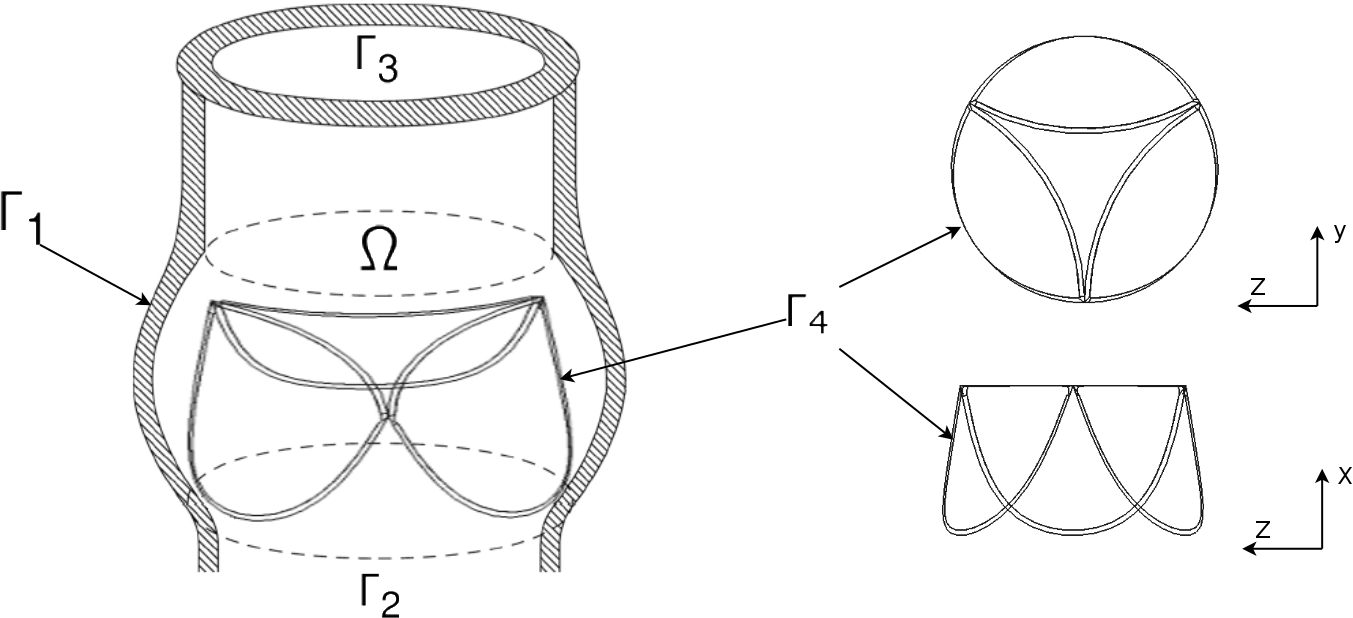
\includegraphics [width=14cm] {aorta_valve_scheme.png}
  \caption{Изображение границ расчетной области} 
  \label{img:aorta_boundaries}
\end{figure}

\subsection*{Моделирование деформации погруженной границы}
Опишем погруженную границу как гибкий несжимаемый материал, который расположен в области $\tilde{\Omega}$,
где $(q, r, s) = \bar{q}$ - криволинейные координаты связанные с материалом так, что зафиксированное значение
$(q, r, s)$ обозначает одну точку этого материала. Пусть $X(q, r, s, t) = X(\bar{q}, t)$ - позиция в декартовых координатах
точки, обозначенной $(q, r, s)$ в момент времени $t$. Тогда обобщая, $X(\bar{q}, t)$ описывает пространственную
конфигурацию всей погруженной границы в момент времени $t$, которая определяет соответствующую энергию деформации
$E[X(\bar{q}, t)]$ в момент $t$. Рассмотрим возмущение $\wp X(\bar{q}, t)$ конфигурации $X(\bar{q}, t)$,
где $\wp$ - оператор возмущения.
%NOTE: перевести точнее, "up to terms of first order" - с точностью первого порядка?
Результирующая деформация упругой энергии, возникшая в результате этого возмущения,
есть линейная функция от возмущения конфигурации, поэтому она может быть записана в форме:
\begin{equation}
\label{eq:elastic_energy_functional}
\wp E[X(\bar{q}, t)] = \int_{\tilde{\Omega}} (-F(\bar{q}, t)) \cdot \wp X(\bar{q}, t)\; d\bar{q}
\end{equation}
где $-F(\bar{q}, t)$ - производная Фреше от $E$, вычисленная для конфигурации $X(\bar{q}, t)$. Физически $F$
можно интепретировать, как плотность силы, которая создается путем деформирования погруженной границы.

Введем два вида погруженных границ:
\begin{itemize}
    \item Неподвижная или малоподвижная граница
    \item Гибкая граница 
\end{itemize}
С помощью неподвижной границы будем моделировать фиксированные участки $\Gamma$, например, фиброзное кольцо,
к которому крепятся лепестки клапана, или стенки кровеносного сосуда, в том случае, если нас не интересуют
их деформации. Гибкие границы предназначены для моделирования подвижных участков $\Gamma$, которые испытывают
наибольшие деформации, например, лепестки клапана. Описанные типы границ обладают разными характеристиками, поэтому
для их описания мы будем использовать разные модели.

Для случая неподвижной границы мы можем использовать простую формулу, выражающую силу $F$ через смещение границы
в момент $t$ относительно исходного положения в момент $t_0$:
\begin{equation}
    \label{eq:simple_force}
    F = k \| X(\bar{q}, t_0) - X(\bar{q}, t) \|
\end{equation}
где $k$ - коэффициент жесткости.

Формула (\ref{eq:simple_force}) не подходит для гибких границ, т.к. позволяет учитывать только небольшие деформации.
Соответствующее уравнение для них может быть получено исходя из следующих соображений.
Как было сказано выше, погруженная граница представлена набором волокон.
Для того, чтобы определить $E$, удобно выбирать лагранжевые координаты $(q, r, s)$ так,
что каждое значение $(q, r)$ параметрически задает какое-либо одно конкретное волокно $s \to X(q^0, r^0, s)$.
В этом случае функционал упругой энергии $E$ можно представить в виде $E = E_s + E_b$,
где $E_s$ - энергия растяжения волокна, $E_b$ - энергия скручивания волокна,
а силу $F$, созданную благодаря деформации, в виде $F = F_s + F_b$.

Как показано в \cite{peskin2002immersed}, \cite{griffith2009simulating} функционал энергии растяжения можно записать в виде:
\begin{equation}
\label{eq:stretching_energy_functional}
E_s = \int_{\tilde{\Omega}} \varepsilon_s \left(\left| \frac{\partial X}{\partial s} \right| \right) d\bar{q}
\end{equation}
а силу $F_s$:
\begin{equation}
\label{eq:stretching_force_density}
F_s = \frac{\partial}{\partial s} \varepsilon_s^{,} \left( \left| \frac{\partial X}{\partial s} \right| \right) \tau
\end{equation}
где $\varepsilon_s$ - локальная энергия растяжения, $\tau$ - единичный тангенциальный вектор для выбранного волокна $s$.
Т.к. напряжение растяжения $T = \varepsilon_s^{,} \left( \left| \frac{\partial X}{\partial s} \right| \right)$, то уравнение (\ref{eq:stretching_force_density})
можно переписать в виде, который соответствует обобщенному закону Гука:
\begin{equation}
\label{eq:stretching_force_density_simplified}
F_s = \frac{\partial}{\partial s} T \tau
\end{equation}

Т.к. площать попреречного сечения сосудов достаточно мала по отношению к их длинне, для моделирования энергии напряжения и 
сил сопротивления скручиванию мы можем воспользоваться уравнением Эйлера-Бернулли \cite{gere1997mechanics}:
% also see here https://en.wikipedia.org/wiki/Euler%E2%80%93Bernoulli_beam_theory
\begin{equation}
    E_b = \frac{1}{2} \int_{\tilde{\Omega}} k \cdot \left| \frac{\partial^2 X^0}{\partial s^2} - \frac{\partial^2 X}{\partial s^2} \right|^2 \; d\bar{q}
\end{equation}

\begin{equation}
    F_b = \frac{\partial^2}{\partial s} \left( k \cdot \left(\frac{\partial^2 X^0}{\partial s^2} - \frac{\partial^2 X}{\partial s^2} \right) \right)
\end{equation}
где $k = E \cdot I$, $E$ - модуль упругости, $I$ - момент инерции поперечного сечения, $\frac{\partial^2 X^0}{\partial s^2}$, $\frac{\partial X}{\partial s^2}$ -
отклонение погруженной границы от равновесного положения в начальный и текущий момент времени.

Таким образом, плотность силы $F$, создаваемая при деформации погруженной границы может быть выражена в виде:
\begin{equation}
    F = \frac{\partial}{\partial s} T \tau + \frac{\partial^2}{\partial s} \left( k \cdot \left(\frac{\partial^2 X^0}{\partial s^2} - \frac{\partial^2 X}{\partial s^2} \right) \right)
\end{equation}

\subsection*{Моделирование взаимодействия}
Как показано в \cite{peskin2002immersed}, для того, чтобы описать взаимодействие потока жидкости и погруженной границы,
необходимо ввести в рассмотрение прямоугольную область $(x, y, z) = \bar{x} \in \tilde{\Omega}$, так что $\Omega \in \tilde{\Omega}$, а также
область $(q, r, s) = \bar{q} \in \Gamma$, которая соответствует точкам погруженной границы в лагранжевых координатах.
В этих областях запишем следующую систему уравнений:
\begin{gather}
    \label{eq:navier_stokes:ibm:motion}
    \frac{\partial \vec{u}}{\partial t} + (\vec{u} \cdot \nabla) \vec{u} = - \frac{1}{\rho} \nabla p + \nabla \sigma + \vec{f}\\
    \label{eq:navier_stokes:ibm:continuity}
    \frac{\partial \rho}{\partial t} + \nabla \cdot (\rho \vec{u}) = 0\\
    \label{eq:interaction:velocity}
    \frac{\partial X}{\partial t}(\bar{q}, t) = \int_{\Omega} \vec{u}(\bar{x}, t) \cdot \delta (x - X(\bar{q}, t))\; d\bar{x}\\
    \label{eq:interaction:force}
    \vec{f}(\bar{x}, t) = \int_{\Gamma} \vec{F}(\bar{q}, t) \cdot \delta (x - X(\bar{q}, t))\; d\bar{q}
\end{gather}

Уравнения (\ref{eq:navier_stokes:ibm:motion}), (\ref{eq:navier_stokes:ibm:continuity}) - это система уравнений Навье-Стокса,
которая используется для моделирования течения жидкости, и полностью записана в эйлеровых координатах $(x, y, z) \in \tilde{\Omega}$.
Уравнения \ref{eq:interaction:velocity},\ref{eq:interaction:force} являются уравнениями взаимодействия жидкости с погруженной границей
и позволяет переходить от эйлеровых к лагранжевым координатам. В уравнениях (\ref{eq:interaction:velocity}), (\ref{eq:interaction:force})
$\delta$ - дельта функция Дирака, $F$ - плотность силы деформации, описанная в предыдущем разделе \textbf{Моделирование деформации погруженной границы}.

Подробное доказательство системы уравнений (\ref{eq:navier_stokes:motion}) - (\ref{eq:interaction:force}) опубликовано в \cite{peskin2002immersed}.
В данной работы мы приведем его краткое описание. Рассмотрим более обший случай,
когда гибкий несжимаемый материал заполняет всю область $\tilde{\Omega}$, т.е. $\tilde{\Omega} = \Gamma$.
Исходя из принципа наименьшего действия, на временном промежутке $(0, T)$ система должна развиваться так, чтобы достигался минимум:
\begin{equation}
    S = \int_0^T L(t) dt
\end{equation}
где $L(t)$ - разница между кинетической и потенциальной энергией, в нашем случае:
% далее везде опущена плотность, надо уточнить
% видимо, дальнейшая цель - взять это уравнение, как данность, и перевести
% все его параметры из лагранжевых в эйлеровы
\begin{equation}
    \label{eq:least_action}
    L(t) = \frac{1}{2} \int \left| \frac{\partial X}{\partial t}(\bar{q}, t) \right|^2 \; d\bar{q} - E(X(\bar{q}, t))
\end{equation}

Т.о. для любого возмущения $\wp X$ требуется:
\begin{equation}
    0 = -\wp S = \int_0^T \int \left( \frac{\partial^2 X}{\partial t^2} - F \right) \cdot \wp X \; d\bar{q} \; dt
\end{equation}

Вводя в рассмотрение скорость жидкости $u$ и скорость деформации $U$:
\begin{gather}
    u(X(\bar{q}, t), t) = \frac{\partial X}{\partial t}(\bar{q}, t) \\
    U(X(\bar{q}, t), t) = \wp X(\bar{q}, t)
\end{gather}
можно показать, что $\wp X$ удовлетворяет условию несжимаемости в лагранжевых координатах, и можно записать следующие уравнения:
\begin{gather}
    \wp X(\bar{q}, t) = \int U(\bar{x}, t) \; \delta(\bar{x} - X(\bar{q}, t)) d\bar{x} \\
    \frac{\partial^2 X}{\partial t^2} \cdot \wp X(\bar{q}, t) = \int  \left(\frac{\partial u}{\partial t} + u \cdot \triangle u \right) U(\bar{x}, t) \; \delta(\bar{x} - X(\bar{q}, t)) d\bar{x}
\end{gather}
Подставляя эти формулы в (\ref{eq:least_action}) получим:
\begin{equation}
    0 = \int_0^T \int \int \left( \frac{\partial u}{\partial t} + u \cdot \triangle u - F(\bar{q}, t) \right) \cdot U(\bar{x}, t) \; \delta(\bar{x} - X(\bar{q}, t)) \; d\bar{x} \; d\bar{q} \; dt
\end{equation}
Произведя замену
\begin{equation}
    f(x, t) = \int F(\bar{q}, t) \; \delta(\bar{x} - X(\bar{q}, t)) \; d\bar{q}
\end{equation}
после ряда преобразований можно завершить переход от лагранжевых переменных к эйлеровым.

Помимо этого, в \cite{peskin2002immersed} показано, что несмотря на отсутствие предположений
о неоднородности плотности жидкости, уравнение:
\begin{equation}
    \frac{\partial \rho}{\partial t} + u \cdot \triangle \rho = 0
\end{equation}
есть следствие приведенной системы уравнений. Метод погруженной границы является следствием описанного случая,
в котором эластичный несжимаемый материал заполняет не всю область $\tilde{\Omega}$, а только часть, и представляет
собой поверхность, погруженную в жидкость.

\subsection*{Численная схема}

Введем в области $\tilde{\Omega}$ сетку $\tilde{\Omega_h}$ с шагами $h_x, h_y, h_z$, в области $\Gamma$ введем сетку $\Gamma_h$
с шагами $h_q, h_r, h_s$. Как показано в \cite{peskin2002immersed}, численно взаимодействие жидкости
и погруженной границы описывается следующими уравнениями:
\begin{gather}
    f(\bar{x}, t_n) = \sum_{\bar{q} \in \Gamma_h}\; F(\bar{q}, t) \delta_h (\bar{x} - X(\bar{q}, t)) \; h_q\; h_r\;  h_s
    f(\bar{x}, t_n) = \sum_{\bar{q} \in \Gamma_h}\; F(\bar{q}, t) \delta_h (\bar{x} - X(\bar{q}, t)) \; h_q\; h_r\;  h_s
\end{gather}

% Численная схема и детали ее реализации

% Подробнее про delta, возможные варианты и условия, которым должно удовлетворять

% Примеры расчетов других авторов, цифры, свои расчеты + сравнение

\bibliography{biblio}
